\documentclass[a4paper]{article}
\usepackage{xeCJK}
\usepackage{verbatim}
\usepackage{graphicx}
\usepackage{hyperref}
\hypersetup{colorlinks}
%\setCJKmainfont{Noto Sans CJK SC}
\setCJKmainfont{宋体}
\setCJKmonofont{微软雅黑}
\pagestyle{plain}
\begin{document}
	\section*{Info}
		\chapter{姓名与通信}
\begin{tabular}{ll}
\hline
  Name : & 周明东 \\
  Tel : & 13922835173 \\
  E-mail : & 505732590@qq.com \\
  GitHub : & \url{https://github.com/catRat} \\
  QQ : & 505732590 \\
  \hline
\end{tabular}

	\section*{Skills}
		\begin{itemize}
\item 熟练使用 Window 操作系统, 了解 Linux 操作系统. 两年 Ubuntu 操作系统使用经验.
\item 熟练使用 Excel, 包括 Excel 的常用函数, Excel 的数据透视表.
\item 熟练使用 Word.
\item 熟练使用 PowerPoint.
\item 熟练使用 R, SPSS, Python.
\item 熟练使用 R 进行数据的清理, 包括
\begin{itemize}
\item 长格式与宽格式的转化,
\item 日期值处理,
\item 字符数据处理,
\end{itemize}
\item 熟练使用 R 的 ggplot2 完成数据可视化工作.
\item 熟练使用 SQL 语言.
\item 熟练使用 R 完成假设检验, 差异分析, 回归分析, 时间序列分析.
\item 了解 Shiny Server, 能够搭建 Shiny Server.
\end{itemize}

	\section*{Education Experience}
		\chapter{教育经历}
\begin{tabular}{ll}
  2013-2017 & 河池学院, 应用统计学, 专业课程是概率论和数理统计 \\
  2012-2013 & 广西百色市祈福高级中学 \\
  2009-2012 & 广西百色市百色民族高级中学  \\
  2007-2009 & 广西那坡县那坡民族初级中学  \\
  2005-2007 & 广西那坡县百合乡百合中学  \\
  1999-2005 & 广西那坡县百合乡那乐村那乐小学 \\
\end{tabular}

	\section*{Work Experience}
		\section{工作经历}
\begin{itemize}
	\item 2017年11月-2018年10月。深圳鸿安货运代理有限公司数据文员。
	\item 2018年11月-2019年6月。深圳裕展精密科技有限公司作业员。
\end{itemize}

	\section*{Present}
		我目前还在公司的岗位中, 公司的岗位交接需要 1 个月的时间. 现在的我积极考虑换工作. 

	\section*{Code Show}
		利用 R 的数据结构和工具, 我能够高效地完成往往需要 VBA 才能完成的工作.
		\verbatiminput{GetCode.R}	
		\verbatiminput{GetId.R}	
		\verbatiminput{Select.R}
		\verbatiminput{blackcat.R}	
	\section*{Graph Show}
		%简单条形图在图 \ref{figure:bara}. 按纵坐标排序后的条形图在图 \ref{figure:barb}. 类别映射到颜色的条形图在图 \ref{figure:bar3}. 类别映射到颜色带有数据标签的条形图在图 \ref{figure:bar4}.
		\begin{figure}
		%\label{figure:bara}
		\begin{center}
		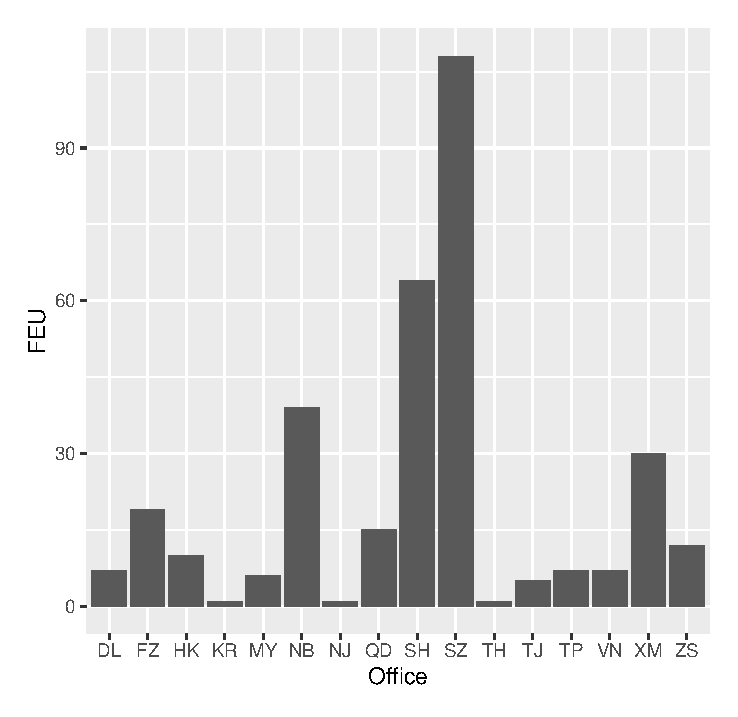
\includegraphics{Rplot01}
		%\caption{简单条形图}
		\end{center}
		\end{figure}
		\begin{figure}
		%\label{figure:barb}
		\begin{center}
		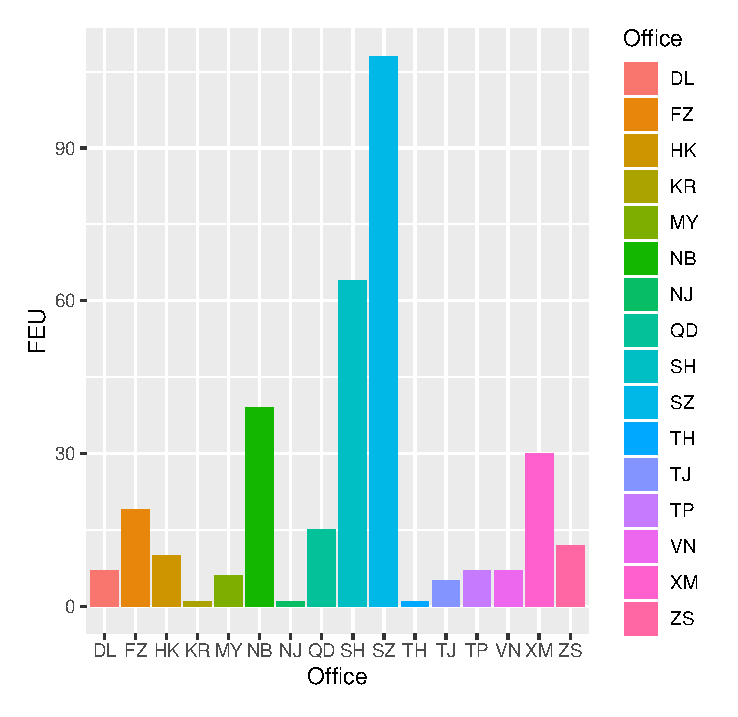
\includegraphics{Rplot02}
		%\caption{按纵坐标排序后的条形图}
		\end{center}
		\end{figure}
		\begin{figure}
		%\label{figure:bar3}
		\begin{center}
		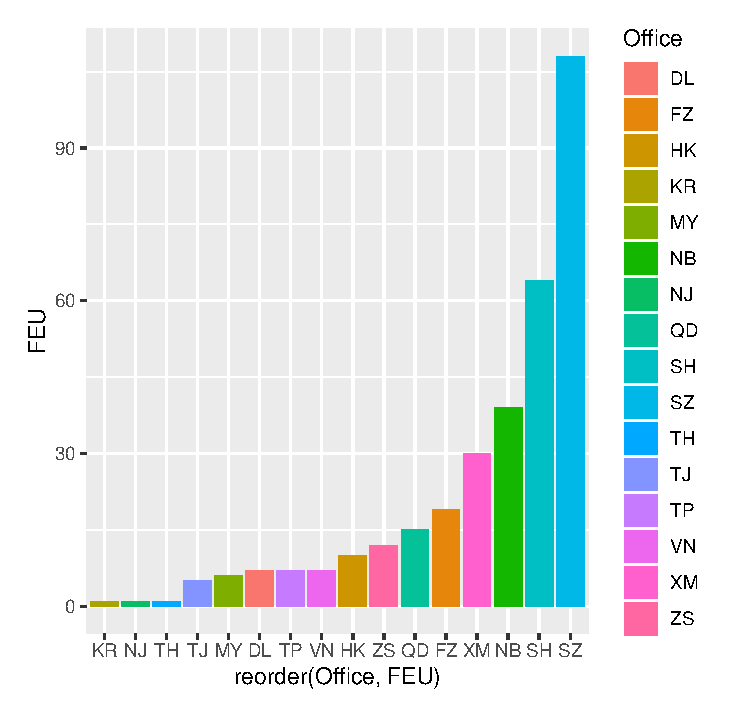
\includegraphics{Rplot03}
		%\caption{类别映射到颜色的条形图}
		\end{center}
		\end{figure}
		\begin{figure}
		%\label{figure:bar4}
		\begin{center}
		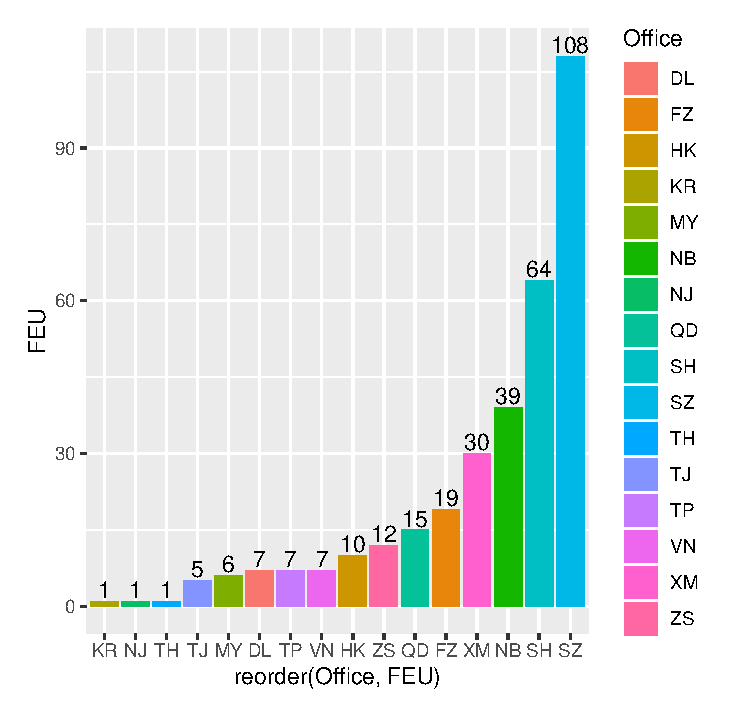
\includegraphics{Rplot04}
		%\caption{类别映射到颜色带有数据标签的条形图}
		\end{center}
		\end{figure}
\end{document}
